\chapter{Results}
\label{chapter6}
\todo{Aim for 6 to 7 pages}

The task of segmenting the aneurysm in the TOF-MRA image is evaluated with the use of three metrics: Dice Similarity Coefficient (DSC), Modified Hausdorff Distance (MHD) (95\textsuperscript{th} percentile), and Volumetric Similarity (VS). The overlap of the prediction and ground truth segmentation map is evaluated using DSC. Compared to DSC, MHD is a distance metric and is sensitive to the overall shape of the segmentation. As the name applies, VS is a measure that considers volumes of the segmentations to indicate similarity. These are reported for the networks described in Chapter \ref{chapter4} -- DeepMedic, and nnU-Net -- and for Triplanar-Net. The metrics are evaluated with using two datasets -- train, and test. The train dataset comprises the publicly available data from the ADAM challenge, and the test dataset the non-publicly available data from the same \cite{Timmins2020}. During training of all networks, the train dataset was split into training and validation sets, with cross-validation, however for methodological reasons when reporting results the train dataset is not split. The results for Triplanar-Net are for the complete framework, i.e. including the classifier.

Each segmented voxel or connected component of voxels is considered a positive detection. A positive detection corresponding to an aneurysm is considered a true-positive finding, whereas a positive detection not corresponding to an aneurysm was considered a false-positive finding. \todo{true negative/false negative?}

The number of parameters of each network, and the inference time for a scan is also reported. Inference time per case is reported without taking into account time required for preprocessing of the data. It should be noted that DeepMedic runs on a Tensorboard backend, whereas the other networks use PyTorch. Therefore \todo{therefore what?}

It is also interesting to further analyze the results with respect to each network: results such as the segmentation performance of true UIAs, and segmentation performance based on size of UIAs are also assessed. It is not possible to perform these assessments on the test dataset as it is not publicly available, so the reporting is done only on the train dataset. 

\section{Metrics}
Results are shown for the segmentation metrics evaluated on the full TOF-MRA volumes in Table \ref{table:metrics_full} for both the train set and the test set. The reported train set result is the average on the validation set over all the folds -- i.e. the available train dataset was manually split into training and validation for 5-fold cross-validation. Figure \ref{fig:results} shows the box plots of the segmentation metrics for the evaluated networks.


\begin{table}[htp]
	\centering
	\begin{tabular}{ l  r r r | r r r }
		\multirow{3}{4em}{} & \multicolumn{3}{ c |}{\textbf{Train}} & \multicolumn{3}{| c }{\textbf{Test}} \\

		& \multirow{2}{2em}{DSC} & MHD & \multirow{2}{2em}{VS} & \multirow{2}{2em}{DSC} & MHD & \multirow{2}{2em}{VS} \\
		& & (mm) & & & (mm) & \\
		\hline

		nnU-Net & \textbf{0.81} & \textbf{0.49} & \textbf{0.89} & \textbf{0.41} & \textbf{8.96} & 0.50 \\
		DeepMedic & 0.11 & 59.70 & 0.33 & 0.07 & 71.41 & 0.34 \\
		Triplanar-Net & 0.14 & 53.90 & 0.42 & 0.11 & 62.35 & \textbf{0.53} \\
	\end{tabular}
	\caption{\todo{caption}}
	\label{table:metrics_full}
\end{table}

\begin{table}[hp]
	\centering
	\begin{tabular}{ l  r r | r r }
		\multirow{3}{4em}{} & \multicolumn{2}{ c |}{\textbf{Train}} & \multicolumn{2}{| c }{\textbf{Test}} \\
		
		& False Positive Count & Sensitivity & False Positive Count & Sensitivity \\
		\hline
		
		nnU-Net & \textbf{0.0} & \textbf{0.96} & \textbf{0.18} & 0.61 \\
		DeepMedic & 99.41 & 0.90 & 118 & \textbf{0.85} \\
		Triplanar-Net & 28.17 & 0.84 & 31.80 & 0.76 \\
	\end{tabular}
	\caption{\todo{caption}}
	\label{table:metrics_detect}
\end{table}

\begin{figure}[htp]
	\centering
	\begin{subfigure}{.6\linewidth}
		\includegraphics[width=\linewidth]{figures/DSC.eps}
	\end{subfigure}
	\begin{subfigure}{.6\linewidth}
		\includegraphics[width=\linewidth]{figures/MHD.eps}
	\end{subfigure}
	\caption[\todo{Mine caption}]{\todo{Caption}}
	\label{fig:results}
\end{figure}
\begin{figure}
	\ContinuedFloat
	\centering
	\begin{subfigure}{.6\linewidth}
		\includegraphics[width=\linewidth]{figures/VS.eps}
	\end{subfigure}
	\begin{subfigure}{.6\linewidth}
		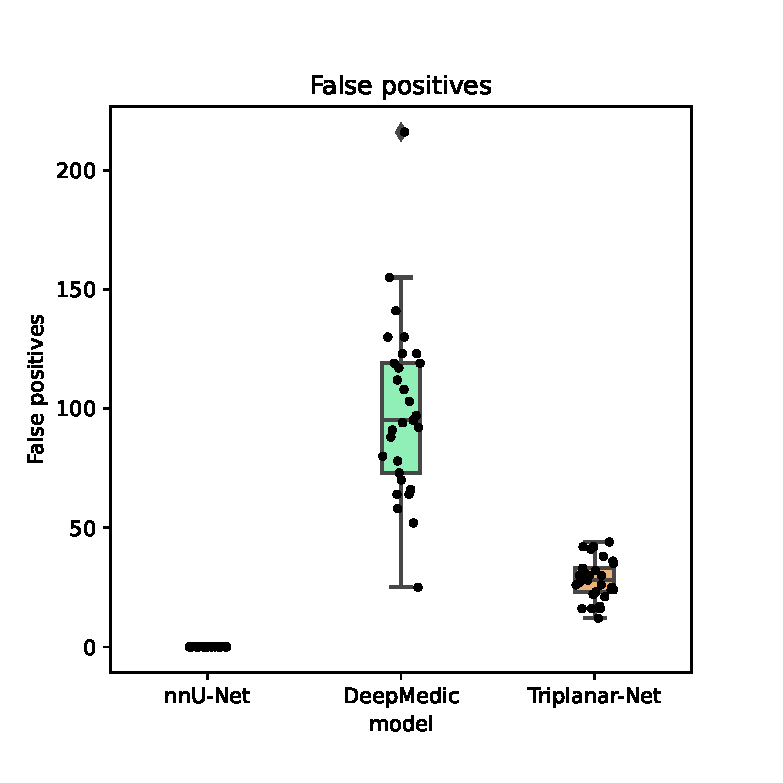
\includegraphics[width=\linewidth]{figures/FalsePositives.eps}
	\end{subfigure}
	\caption[\todo{Mine caption}]{\todo{Caption}}
	\label{fig:results_cont}
%	\caption[\todo{Mini caption}]{\todo{Caption}}
%	\label{fig:results_detect}
\end{figure}
\begin{figure}
	\ContinuedFloat
	\centering
	\begin{subfigure}{.6\linewidth}
		\includegraphics[width=\linewidth]{figures/Sensitivity.eps}
	\end{subfigure}
	\caption[\todo{Mini caption}]{\todo{Caption}}
	\label{fig:results_cont_cont}
\end{figure}

\section{Further evaluation}

\subsection{Inference}
Inference time and number of parameters of the three network architectures are shown in \ref{table:inference}; inference time is a very dependent result and to attempt to keep it as unbiased and normalized as possible, for all networks inference was done on an NVIDIA P100 GPU under equivalent conditions. The mean inference time is reported in seconds and calculated by taking an average of the time required for the forward pass of the network over all train data.

\begin{table}[h]
	\centering
	\begin{tabular}{l r r }
		& parameters & mean inference time (s) \\
		\hline
		nnU-Net & 178297920 & 203 \\
		DeepMedic & \textbf{1178100} & 175 \\
		Triplanar-Net & 1478264 & \textbf{35} \\
	\end{tabular}
	\caption{\todo{caption}}
	\label{table:inference}
\end{table}

\subsection{Segmentation results of true UIAs}
\todo{segmentation results of true UIAs, i.e. ignore false positive detections}

\begin{table}[h]
	\centering
	\begin{tabular}{ l  r r r }
%		\multirow{3}{4em}{} & \multicolumn{3}{ c }{\textbf{Train}} \\
%		
		& \multirow{2}{2em}{DSC} & MHD & \multirow{2}{2em}{VS} \\
		& & (mm) & \\
		\hline
		%		3D U-Net & 0. & 0. & 0. & 0. & 0. & 0. \\
		nnU-Net & 0. & 0. & 0. \\
		DeepMedic & 0. & 0. & 0. \\
		Triplanar-Net & 0. & 0. & 0. \\
	\end{tabular}
	\caption{\todo{caption}}
	\label{table:metrics_pos}
\end{table}

\subsection{Performance on negative scans}

%\subsection{Intra-subject analysis}

\subsection{Qualitative results}

\todo{intra-subject analysis}

\todo{Qualitative results. MITK?}